\begin{figure*}[hbtp]
  \centering
  \subfigure[Phase split]{
    \label{fig:leiden-splits--phase}
    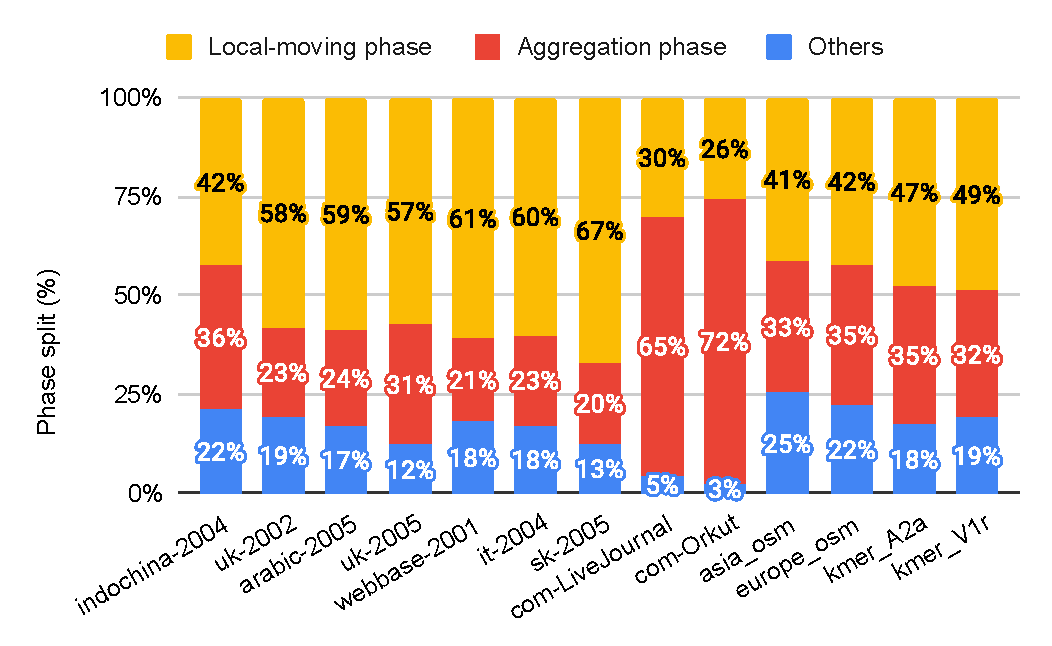
\includegraphics[width=0.48\linewidth]{out/leiden-phases.pdf}
  }
  \subfigure[Pass split]{
    \label{fig:leiden-splits--pass}
    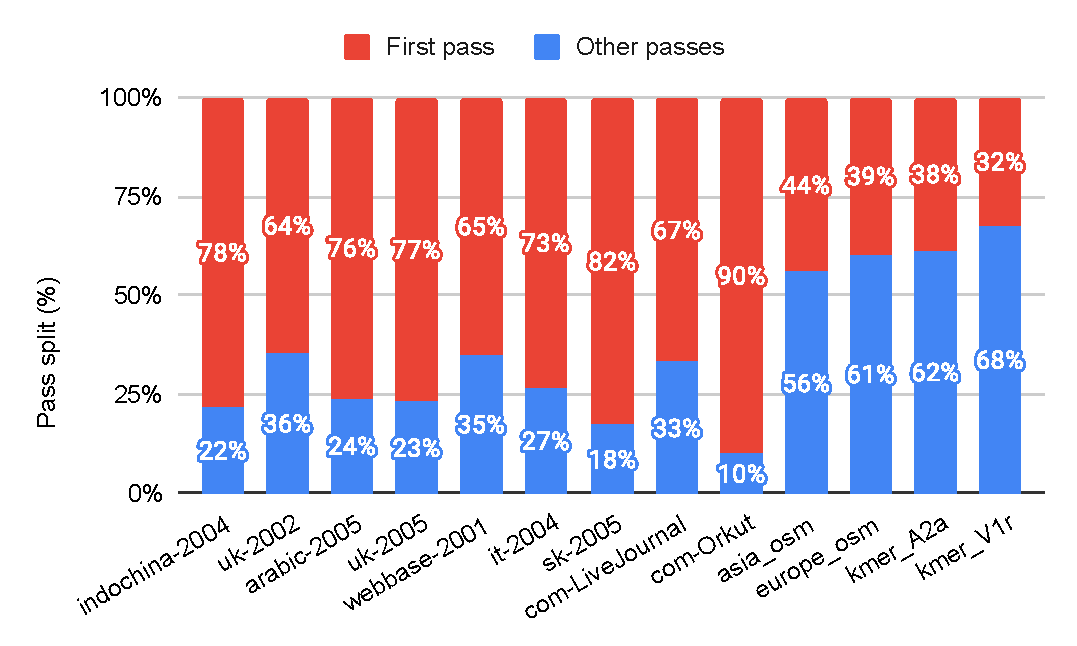
\includegraphics[width=0.48\linewidth]{out/leiden-passes.pdf}
  } \\[-2ex]
  \caption{Phase split of \textit{GVE-Leiden} shown on the left, and pass split shown on the right for each graph in the dataset.}
  \label{fig:leiden-splits}
\end{figure*}
